\chapter{Asservissement}
    Que ce soit en robotique ou dans différents processus industriels, il est souvent indispensable de contrôler certaines grandeurs physiques.
    On appelle \textbf{asservissement} d'une grandeur l'ensemble des moyens permettant de contrôler \textbf{automatiquement} cette grandeur.\\
    Celui-ci peut être mis en place soit au moyen d'un \textit{système en boucle ouverte}, c'est a dire en calculant une commande sans prendre en compte la réponse du système: le système nécessite alors une parfaite modélisation, nous ne nous attarderons donc pas sur ce type d'asservissement.\\
    L'asservissement dont nous allons parler se place dans le cas d'un \textbf{système en boucle fermée} ou \textbf{système à contre réaction négative}, qui, contrairement à son homologue ouvert, mesure la réaction du système pour adapter la commande. Toute la difficulté est alors de réussir à déterminer la fonction permettant d'adapter la commande de sortie en fonction de l'objectif voulu et du résultat mesurée.\\
    Le correcteur \textit{PID} est un exemple de système à boucle fermée permettant d'asservir efficacement une grandeur. C'est le correcteur le plus utlisié, qui a largement fait ses preuves dans l'industrie.
    \begin{figure}[h]
        \centering
        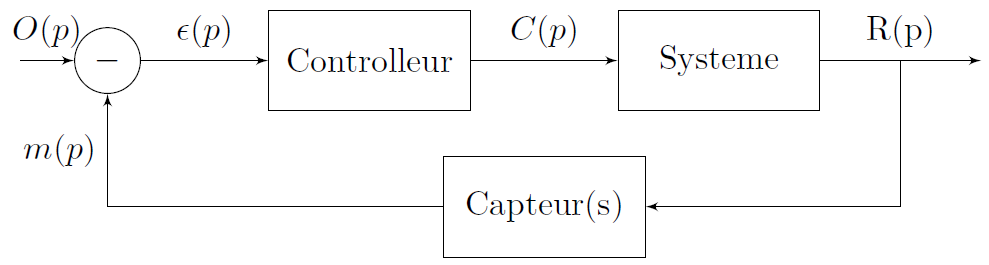
\includegraphics[scale=0.35]{assets/ASSERV.png}
        \caption{Représentation d'un système asservi en boucle fermée}
    \end{figure}


    \newpage
    \section{Correcteur PID}
        Le correcteur PID est un système à contre réaction \textbf{négative}, il calcule donc une commande en fonction de l'erreur $\epsilon$ de la grandeur, c'est à dire la différence entre la valeur voulue (i.e l'objectif) $O$, et valeur mesurée $m$.
        \begin{equation}
            \epsilon (t) = O(t) - m(t)
        \end{equation}
        La commande de sortie, passée au travers d'un correcteur PID, qu'on note $C(t)$, consiste en une somme de trois termes: une réponse proportionnelle à l'erreur, une réponse proportionnelle à la somme des erreurs, et une réponse proportionnelle à l'évolution de l'erreur. Une traduction quasi-litéralle de cette définition nous donne la relation suivante:
        \begin{equation}
            C(t) = f(\epsilon(t)) = K_p . \epsilon(t) + K_i . \int_{0}^{t}\epsilon(\tau).d\tau + K_d . \frac{d\epsilon}{dt}(t)
        \end{equation}
        Ou plus simplement\footnote{Les relations mettant en jeux des intégrales et des dérivées sont plus simples à exprimer dans le domaine de Laplace} dans le domaine de Laplace:
        \begin{equation}
            C(p) = f(\epsilon(p)) = K_p . \epsilon(p) + K_i . \frac{\epsilon(p)}{p} + K_d.p.\epsilon(p)
        \end{equation}
        Ce que l'on peut résumer à l'aide du schéma-bloc suivant:
        \begin{figure}[h]
            \centering
            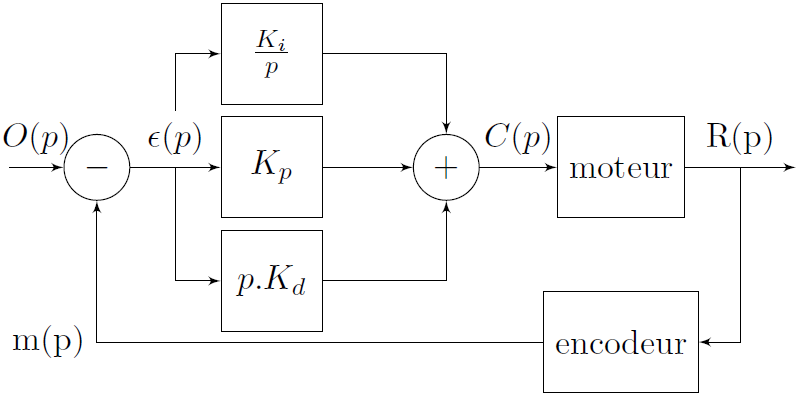
\includegraphics[scale=0.35]{assets/PID.png}
            \caption{Représentation d'un correcteur PID}
        \end{figure}

        \newpage
        \subsection{Influence des coefficients}
            Dans cette section, allons présenter l'influence des différents coefficients sur le système. En guise d'introduction à chacun d'eux, nous allons faire le parallèle avec un système (une voiture) et son correcteur pouvant être assimilé à un PID (un conducteur). On se place dans le cas ou sur une route, le conducteur décide d'être éxactement à la limite de la distance de sécurité de la voiture d'en face.

            \subsubsection{Réponse proportionnelle}
                \textit{«Plus je suis loin de la limite, plus je dois appuyer sur la pédale d'accélération.»}\\
                Le terme proportionnel permet de répondre aux grandes inerties du système, et diminue le temps de montée en donnant l'essentiel de la puissance au moteur: plus l'erreur est grande, plus la réponse est importante. La valeur de $K_p$ est proportionnelle à la vitesse de réaction du système. L'erreur statique est réduite avec l'augmentation de $K_p$, cependant le système perd en stabilité. En cas de $K_p$ démesuré, le système oscille et ne trouve jamais stabilité.\\
                Dans le cas d'un moteur, une variation trop faible de tension ne fait plus varier sa vitesse. Ainsi lorsque l'erreur devient trop faible, le terme proportionel ne permet pas de combler une erreur statique qui est d'autant plus faible que $K_p$ est grand.

            \subsubsection{Réponse intégrale}
                \textit{«Moins j'accélère pour une pression de la pédale d'accélération donnée, plus je dois appuyer sur la pédale.»}\\
                Le terme intégral fait la somme algébrique des erreurs. Il permet ainsi de donner une réponse de plus en plus forte à mesure que le système persiste dans son erreur. Il complète ainsi le terme proportionel, car permet de combler l'erreur statique laissée par ce dernier en régime permanent.\\
                Augementer $K_i$ permet de diminuer l'impact de faibles perturbations, augemente la précision du système en régime permanent. Un $K_i$ trop important peut cependant augementer le dépassement de la consigne «overshoot», et causer d'oscillations semblables à celles du $K_p$ en cas de valeur démesurée.

            \subsubsection{Réponse dérivée}
                \textit{«Plus j'accélère vite et que je me rapporoche de la limite (et risque donc de la dépasser), moins je dois appuyer sur la pédale.»}\\
                L'action du terme dérivé dépend du signe et de la vitesse de variation de l'erreur. Sa valeur va donc s'opposer à la réponse proportionnelle et intégrale. Elle devient importante lorsque l'erreur faiblit grandement et que le terme proportionnel continue à donner de grandes valeurs: elle freine le système empéchant le dépassement de la consigne et diminuant les petites oscillations qui ralentissent la stabilisation du système. $K_d$ compense donc $K_p$ lorsque l'erreur faiblit, on peut ainsi pousser $K_p$ pour limiter l'erreur statique quitte à dépasser la consigne, puis compenser ce dépassement en augementant $K_d$.

        \newpage

        \subsection{Réglage des coefficients}
            Régler les coefficients représente la majeure difficulté de la mise en place d'un asservissement PID. On s'intéresse ici uniquement à l'asservissement d'un moteur (à courant continu, ou pas).

            \subsubsection{Méthode théorique: Modélisation du système}
            Dans un premier temps, il est toujours intéressant de s'intéresser à la réponse théorique du système. Cette méthode n'est donc pas une méthode complète en soit, mais juste un outil permettant de "dégrossir" les coefficients avant de les affiner sur le système final.\\
            Les démonstrations des fonctions de transfert ci-dessous ne seront pas développées ici, car elle ne font pas l'objet de ce document. En effet, seul le modèle final et son utilisation nous intéresse.\\
            La fonction de transfert entre la vitesse angulaire de sortie et la tension d'entrée d'un moteur peut être modélisée comme un filtre du second ordre:
            \begin{equation}
                H(p) = \frac{\omega(p)}{U(p)} = \frac{A}{1 + \frac{2.\xi}{\omega_0} + \frac{1}{\omega_0^2}.p^2}
            \end{equation}
            Avec:
            \begin{itemize}
                \item $\omega(p)$ Vitesse de rotation du rotor
                \item $U(p)$ Tension appliquée au moteur
                \item $A = \frac{1}{K_e}$ Gain statique
                \item $\omega_0 = \sqrt{\frac{K_e.K_c}{L.J_T}}$ Pulsation propre
                \item $K_e/K_c$ Constante de vitesse/couple
                \item $J_T$ Moment d'inertie apporté au rotor
            \end{itemize}

            \paragraph{Moteur à courant continu}{
                \begin{itemize}
                    \item $\xi = \frac{R}{2}\sqrt{\frac{J_T}{K_e.K_c.L}}$ Facteur d'amortissement
                    \item $R$ Résistance au bornes du moteur
                    \item $L$ Inductance du moteur
                \end{itemize}
            }


            \paragraph{Moteur sans balais}{
                \begin{itemize}
                    \item $\xi = \frac{3R}{2}\sqrt{\frac{J_T}{K_e.K_c.L}}$ Facteur d'amortissement
                    \item $Ke = 0,0605.K_t$
                    \item $R$ Résistance phase-à-phase
                    \item $L$ Inductance phase-à-phase\\
                \end{itemize}
            }
            Il est possible de modéliser le moment d'inertie $J_T$ perçu par le moteur sur son arbre dans le cas d'une utilisation sur un robot de masse $M$ en connaissant le rayon des roues $R$.
            \begin{equation}
                J_T = M.R^2
            \end{equation}

            \newpage
            \subsubsection{Méthode empirique 1: dite de «Ziegler-Nichols»}
                La méthode de Ziegler-Nichols ne nécessite aucune modélisation au préalable, seule une batterie d'éssais expérimentaux souvent automatisables est nécessaire.\\
                Le principe est de fixer $K_i$ et $K_d$ à 0, puis d'augementer $K_p$ jusqu'à obtenir une réponse oscillante en régime permanent. On mesure alors la période $T_osc$ de cette réponse à $(K_p)_{lim}$.\\
                Les coefficients sont déduits de ces deux mesures par les relations suivantes:
                \begin{equation}
                \begin{cases}
                    K_p = 0.6 . (K_p)_{lim}\\
                    K_i = \frac{1}{0.5 . T}\\
                    K_d = 0.125 . T
                \end{cases}
                \end{equation}
                Les coefficients déduits sont assez polyvalents car ils proposent un bon compromis entre rapidité, dépassement de la consigne, stabilité, et précision. Néammoins, selon la spécification de la réponse désirée, il est possible d'ajuster les différents coefficients à la main. Par exemple, dans le cas de l'asservissement d'un robot, on va vouloir limiter au maximum le dépassement de consigne et donc baisser $K_p$.

            \subsubsection{Méthode empirique 2: dite «À la main»}
                Cette dernière méthode est utile lorsque l'on a des besoins spécifiques quant à la réponse du système. Par exemple, sur un asservissement en position, on peut vouloir complètement éliminer le dépassement de la consigne (il peut être critique d'aller trop loin et de déplacer un objet à la coupe de France !), quitte à avoir un temps de stabilisation plus long. Dans ce cas là, un asservissement de type PD est recommendable. Le principe est de faire varier $K_p$ jusqu'à qu'il y ai dépassement de consigne, puis de compenser en augmentant $K_d$ jusqu'à élimination de l'erreur statique.

    \section{Asservissement en vitesse}
        Première manière de contrôler le déplacement du robot: on asservit indépendemment chaque moteur en vitesse.\\
        Incovénient: pour aller à une position donnée, il faut donc intégrer numériquement les consignes de vitesse.
    \subsubsection{Code d'exemple}
            \begin{lstlisting}[language=JavaScript]
function velocityControl() {
    let velocity = encoder.getTicks(); // Vitesse en implusion par DeltaT
    encoder.resetTicks();

    previousVelocityError = velocityError;
    velocityError = velocityObjective - velocity;

    let derivative = velocityError - previousVelocityError; // On inclut le 1/DeltaT dans K_d
    integral += velocityError;

    velocityCommand = kp * velocityError + ki * integral + kd * derivative;

    return velocityCommand;
}
            \end{lstlisting}

    \newpage
    \section{Asservissement en position}
        Asservir indépendemment chaque moteur en position permet de résoudre le  problème d'intégration numérique. Par contre, la vitesse n'étant plus asservie, l'accélération peut être beaucoup trop grande, on s'expose alors à des risques de dérapages.
    \subsubsection{Code d'exemple}
            \begin{lstlisting}[language=JavaScript]
function positionControl() {
    position += encoder.getTicks(); // Position en ticks
    encoder.resetTicks();

    previousPositionError = positionError;
    positionError = velocityObjective - velocity;

    let derivative = positionError - previousPositionError; // On inclut le 1/DeltaT dans pKd
    integral += positionError;

    positionCommand = pKp * positionError + pKi * integral + pKd * derivative;

    return positionCommand;
}
            \end{lstlisting}

    \section{Asservissement en vitesse et en position}
        Réunir à la fois un asservissement en vitesse et en position permet de réunir le meilleur des deux mondes. On peut controller la vitesse, et donc l'accélération tout en se passant d'intégration numérique grace à l'asservissement en position.\\
        Un premier asservissement en position va donner une consigne de vitesse, qui après traitement algorithmique pour écrêter vitesse et accélération, va servir de consigne pour un deuxième asservissement en vitesse. On est donc capable de faire atteindre aux moteurs n'importe quelle position tout en controlant la vitesse ainsi que l'accélération à laquelle ils y vont.

        \subsubsection{Choix du profil de vitesse}
        Le profil de vitesse adopté est trapézoïdal. On commence par une phase d'accélération jusqu'à une vitesse de croisière, puis une déccélération jusqu'à atteindre la position voulue. L'avantage est de ne pas brusquer les moteurs, de ne pas déraper au démarrage et de ne pas dépasser l'objectif de position par inertie.

        \begin{figure}[h]
            \centering
            
\begin{tikzpicture}
% horizontal axis
\draw [->] (0,0) -- (8cm,0) node[below] {$t$};

% vertical axis
\draw[->] (0,0) -- (0,4cm) node[anchor=east] {$V$};

\foreach \x in {0,1,2,3,4, 5, 6, 7}
    \draw (\x cm,1pt) -- (\x cm,-1pt) node[anchor=north] {};
\foreach \y in {0,1,2,3}
    \draw (1pt,\y cm) -- (-1pt,\y cm) node[anchor=east] {};

% nominal speed
\draw[dotted] (2,0) -- (2,4);
\draw[dotted] (5,0) -- (5,4);

% Us
\draw[thick] (0,0) -- (2,2) -- (5,2) -- (7,0);
\draw (0.7,1.5) node {$A_{max}$}; %label
\draw (3.5,2.5) node {$V{max}$}; %label
\draw (6.3,1.5) node {$-A_{max}$}; 

\end{tikzpicture}
            \caption{Profil de vitesse trapézoïdal}
        \end{figure}

        \newpage

        Au niveau de l'algorithme, on tronque juste la valeur de la vitesse si elle dépasse une valeur $V_{max}$. On fait de même avec l'accélération en tronquant sa valeur absolue à $A_{max}$.
        \subsubsection{Code d'exemple}
            \begin{lstlisting}[language=JavaScript]
function motionControl() {
    previousVelocityObjective = positionCommand;
    velocityObjective = positionControl();

    // Ecretage de la vitesse
    if (Math.abs(velocityObjective) > maxVelocity) {
        velocityObjective = sign(velocityObjective) * maxVelocity;
    }

    let acceleration = velocityObjective - previousVelocityObjective;
    // Ecretage de l'acceleration
    if (Math.abs(acceleration) > maxAcceleration) {
        velocityObjective = previousVelocityObjective + sign(acceleration) * maxAcceleration;
    }

    motor.run(velocityControl());
}
            \end{lstlisting}

    \newpage
    \section{Asservissement polaire}
        Jusqu'à présent, tous les types d'asservissement proposés se faisaient sur une ou deux grandeurs, indépendemment sur chaque moteur. Il est possible de travailler sur des grandeurs «couplée», réunissant les informations fournies par les deux moteurs.\\

        Pour un robot, il peut être intéressant d'asservir sur la position et l'orientation. L'intérêt est de pouvoir facilement envoyer le robot à une une position $(x, y, \theta)$, sans avoir à faire du traitement algorithmique pour déterminer les consignes de position à envoyer à chaque moteur comme dans un asservissement position ou position/vitesse.\\
        On a donc en tout quatre controlleurs PID: deux pour un asservissement position/vitesse sur la vitesse de déplacement du robot, et deux pour un asservissement position/vitesse sur la vitesse angulaire du robot.\\
        Les grandeurs mesurées ne sont plus directement les impulsions d'encodeur, mais les variations de vitesse et de vitesse angulaire calculées par l'odométrie et décrites par les relations \eqref{dTAU} et \eqref{dTHETA} pour les PID de vitesse, et l'orientation/distance globale pour les PID de distance.

        \subsubsection{Code d'exemple}
            \begin{lstlisting}[language=JavaScript]
function robotControl() {
    /*
        Quadruple asservissement position/vitesse sur la distance et l'angle
        calcules par l'odometrie
    */
    let distanceVelocityCommand = distanceMotionControl();
    let orientationVelocityCommand = orientationMotionControl();

    /*
        Signe arbitraire. On part du principe que l'angle est calcule avec la
        difference entre la position gauche et droite
     */
    leftMotor.run(distanceVelocityCommand - orientationVelocityCommand);
    rightMotor.run(distanceVelocityCommand + orientationVelocityCommand);
}
            \end{lstlisting}
